%!TEX root=main.tex
\section[Aufbau des Auges\hfill Aufbau der Materie]{Aufbau des Auges\\{\normalsize Aufbau der Materie}}
\label{sec:auge}
% Das visuelle System dient zur Verarbeitung visueller Information und umfasst Auge, Sehnerv und Teile des Gehirns.

% \subsection{Das Auge}
Das Auge ähnelt in seiner Funktion einer Kamera. Die Linse (das Objektiv) sammelt Lichtstrahlen und projiziert diese als auf dem Kopf stehendes gespiegeltes Bild auf die Netzhaut (den Film). Da der Abstand zwischen Linse und Netzhaut (die Bildweite) unveränderlich ist, muss die Brechkraft (Brennweite) der Augenlinse angepasst werden. Diese Anpassung nennt man \textit{Akkommodation}.

\begin{figure}
	\centering
	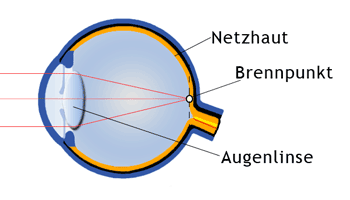
\includegraphics[width=4.5cm]{images/auge.png}
	\caption{Auge \cite{abadi:fehlsichtigkeit}}
\end{figure}

Die Projektion wird von lichtempfindlichen Sehzellen wahrgenommen und von \textit{Photorezeptoren} in elektrische Nervenimpulse umgewandelt. Diese werden in zwei Arten unterschieden: Die \textit{Zapfen} dienen zur Interpretation von Farbe, während die \textit{Stäbchen} zwischen hell und dunkel unterscheiden.

\begin{figure}
	\centering
	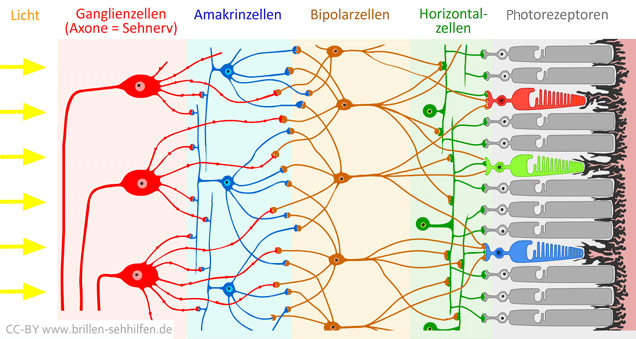
\includegraphics[width=10cm]{images/netzhaut.png}
	\caption{Sehzellen der Netzhaut \cite{bs:auge}}
\end{figure}

Die Zapfen werden wiederum in drei Zelltypen unterschieden, welche jeweils auf Licht einer bestimmten Wellenlänge reagieren. 

\begin{figure}
	\centering
	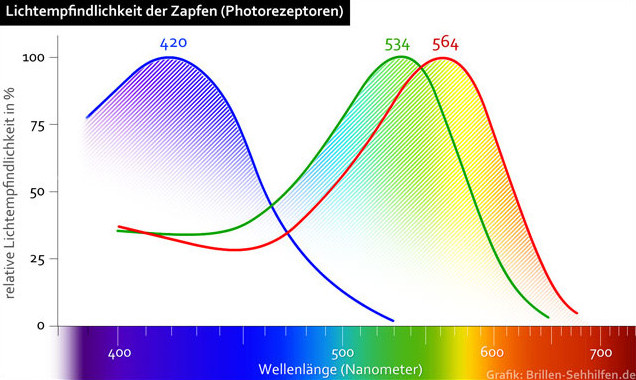
\includegraphics[width=10cm]{images/zapfen.jpg}
	\caption{Farbwahrnehmung der Zapfen \cite{bs:auge}}
\end{figure}

% TODO: Brechzahl, Brechungsindex, optische Dichte
% TODO: Streuung vs. Brechung
